\documentclass [10pt]{book}
\oddsidemargin=0.0cm
\textwidth=16.5cm
\textheight=22.8cm
\topmargin=-1.0cm
\usepackage[utf8]{inputenc}
\usepackage{booktabs}
\usepackage{fancyhdr}
\usepackage{multicol}
\usepackage{mathtools}% Loads amsmath
\usepackage{flowchart}
\usepackage{xcolor}
\usepackage{lipsum}
\usepackage{graphicx}
\usepackage{float}
\usepackage{geometry}
\renewcommand*\contentsname{Contents}
\definecolor{namecolor}{cmyk}{1,.50,0,.10}
\definecolor{titlepagecolor}{cmyk}{1,.21,0,.64}
\definecolor{mint}{cmyk}{.1310,0,.1071,.0118}
\definecolor{teal}{cmyk}{.8523,.0909,.0000,.6549}
\renewcommand{\thesection}{\arabic{section}}
\renewcommand{\headrulewidth}{3pt}% 2pt header rule
\renewcommand{\headrule}{\hbox to\headwidth{%
  \color{titlepagecolor}\leaders\hrule height \headrulewidth\hfill}}
\pagestyle{fancy}
\fancyhf{}
\fancyhead[LE]{\color{teal}\hspace*{-0.2\headwidth}\colorbox{mint}{\makebox[\dimexpr0.2\headwidth-2\fboxsep][c]{\strut\thepage}}%
               \color{white}\colorbox{titlepagecolor}{\makebox[\dimexpr\headwidth-2\fboxsep][l]{Section \strut\thesection}}}
\fancyhead[LO]{\color{white}\colorbox{titlepagecolor}{\makebox[\dimexpr\headwidth-2\fboxsep][r]{Section \strut\thesection}}%
                \color{teal}\colorbox{mint}{\makebox[\dimexpr0.2\headwidth-2\fboxsep][c]{\strut\thepage}}}
\renewcommand{\headrulewidth}{0pt}
%\lhead{\fancyplain{}{\leftmark }}
%\rhead{\fancyplain{}{Alarm Clock}}
%\renewcommand{\headrulewidth}{1pt}
\lfoot{}
\usepackage{listings}
\usepackage{multicol}

% the following is needed for syntax highlighting
\usepackage{color}
\definecolor{dkgreen}{rgb}{0,0.6,0}
\definecolor{gray}{rgb}{0.5,0.5,0.5}
\definecolor{mauve}{rgb}{0.58,0,0.82}
\lstset{ %
%language=[C]{Assembler},       % the language of the code
basicstyle=\scriptsize,         % the size of the fonts that are used for the code
numbers=left,                   % where to put the line-numbers
numberstyle=\tiny\color{gray},  % the style that is used for the line-numbers
stepnumber=1,                   % the step between two line-numbers. If it's 1, each line
% will be numbered
numbersep=5pt,                  % how far the line-numbers are from the code
backgroundcolor=\color{white},  % choose the background color. You must add \usepackage{color}
showspaces=false,               % show spaces adding particular underscores
showstringspaces=false,         % underline spaces within strings
showtabs=false,                 % show tabs within strings adding particular underscores
frame=single,                   % adds a frame around the code
rulecolor=\color{white},        % if not set, the frame-color may be changed on line-breaks within not-black text (e.g. commens (green here))
tabsize=2,                      % sets default tabsize to 2 spaces
captionpos=b,                   % sets the caption-position to bottom
breaklines=true,                % sets automatic line breaking
breakatwhitespace=false,        % sets if automatic breaks should only happen at whitespace
title=\lstname,                 % show the filename of files included with \lstinputlisting;
% also try caption instead of title
keywordstyle=\color{blue},          % keyword style
commentstyle=\color{gray},       % comment style
stringstyle=\color{mauve},         % string literal style
escapeinside={\%*}{*)},            % if you want to add a comment within your code
morekeywords={*,...}               % if you want to add more keywords to the set
}
% facilitates the creation of memory maps. Start address at the bottom, end address at the top.
% Addresses will be print with a leading '0x' and in upper case.
% syntax: \memsection{end address}{start address}{height in lines}{text in box}
\newcommand{\memsection}[4]{
  \bytefieldsetup{bitheight=#3\baselineskip}	% define the height of the memsection
  \bitbox[]{8}{
    \texttt{0x\uppercase{#1}}	 % print end address
    \\ \vspace{#3\baselineskip} \vspace{-2\baselineskip} \vspace{-#3pt} % do some spacing
    \texttt{0x\uppercase{#2}} % print start address
  }
  \bitbox{16}{#4} % print box with caption
}

% Start the document
\begin{document}
  % tite page
  \begin{titlepage}
\vspace*{\fill}
\pagecolor{titlepagecolor}
\color{white}

\begin{center}
\begin{figure}[!h]
   \centerline{\includegraphics[scale=0.6]{images/sp-logo-transparent}}
\end{figure}
\end{center}
\begin{center}
	%\LARGE\textsf{A web based 3D printer management and environmental monitoring system.}

	\vspace{1.8em}

	\Huge\textbf{\texttt{User Documentation}} \textcolor{titlepagecolor!20}{\textsf{}}
\end{center}

\vspace*{\fill}
\end{titlepage}


  % page intentionaly left blank bg white
  \pagecolor{white}

  % table of contents
  \tableofcontents

  \newpage

  \section{Overview}
  \begin{center}
   	\includegraphics[scale=0.25]{images/flow.png}
  \end{center}
  The stratus print system consists of four main parts. The web page, hub, nodes and printer
  control box. The web page is where the system is controlled. From the web page you can set up
  the system, monitor printers and control print jobs. The hub is the heart of the system. It is
  used to relay information from the printer control box and the nodes to the web page. The printer
  control box does what the name implies. Allows control of the printer through the web site as well
  as provides a button for canceling and completing print jobs.

  \subsection{General Work flow}
    \begin{enumerate}
      \item Upload a print job trough the web interface
      \item When the job is finished printing the red light on the printer control box
      will blink. This means it is safe to clean off the print service and prepare the
      surface for the next print job.
      \item When the surface is ready for the next print job press the flashing red button \textbf{ONCE} to start the next job in the queue.  \emph{Wait 20 seconds for the light to stop blinking after pressing the button.  It may take up to 20 seconds for the light to stop blinking while the next job in the queue is being processed!} 
    \end{enumerate}
  \newpage
    \section{Hub}
  \subsection{Set up}
    \begin{enumerate}
      \item

      \item

      \item
    \end{center}


    \end{enumerate}

  \subsection{Troubleshooting}

  \begin{enumerate}
    \item
    \item
  \end{enumerate}


  \newpage
    \section{Nodes}
  \subsection{Set up}
    \begin{enumerate}
      \item Ensure the node is plugged in to an outlet, and the switch is in the \textbf{ON} position 
      (it should be ON by default).
      The red light will be illuminated on the node when it is on.\\ 
TODO ADD GRAPHIC NODE ON\\
      \begin{center}
      \includegraphics[scale=1]{images/Now-Later.png}
    \end{center}

      If the node has already been activated, you are done with this section, proceed to the Web section (Part 3).

      \item If this is the first time the node is being connected to the hub,
      you will need to activate it. To do this you will need a device
      capable of connecting to a wifi network, such as a smart phone, tablet, or computer.\\
      \\ 
      Under wifi networks, you should see a network called \textbf{SetUpGadget\_FPFDHI}\\
      Note that the "FPFDHI" can be any sequence of letters and is specific to the node. Connect to that network. 
      \emph{Once connected you may get a warning that the network does not have access
      to the internet. That is normal, proceed anyway.}

      \item Open your browser and navigate to \textbf{192.168.4.1}

      \begin{center}
      \includegraphics[scale=1]{images/ip-enter.png}
    \end{center}  

      This will bring up a wifi login page:

      \begin{center}
      \includegraphics[scale=0.25]{images/wifi-login.png}
    \end{center}
      Type the information as follows (\emph{case matters, use both upper- and lower-case letters as indicated}):\\
      The wifi name is \textbf{StratusPrint}\\ 
      The password is \textbf{FusRoDah}\\
      \emph{This is the default wifi name and password for the hub and can be changed later.}\\


      \item Click the save button. If successful, the \textbf{SetUpGadget\_FPFDHI} network should disappear
      from your visible networks. This may take 1-3 minutes. If the network is still
      visible, please turn your wifi off and on again to confirm it remains visible. If it is still there,
      please start over from step 2 and make sure you correctly input all information.

    \end{enumerate}

  \subsection{Sensors}
  \emph{This section provides more information on the sensors currently attached to the node, and 
      how to add new sensors.  You may skip this section if you are not adding or replacing sensors.}\\
  \subsubsection{Node Pinout}
  \begin{center}
        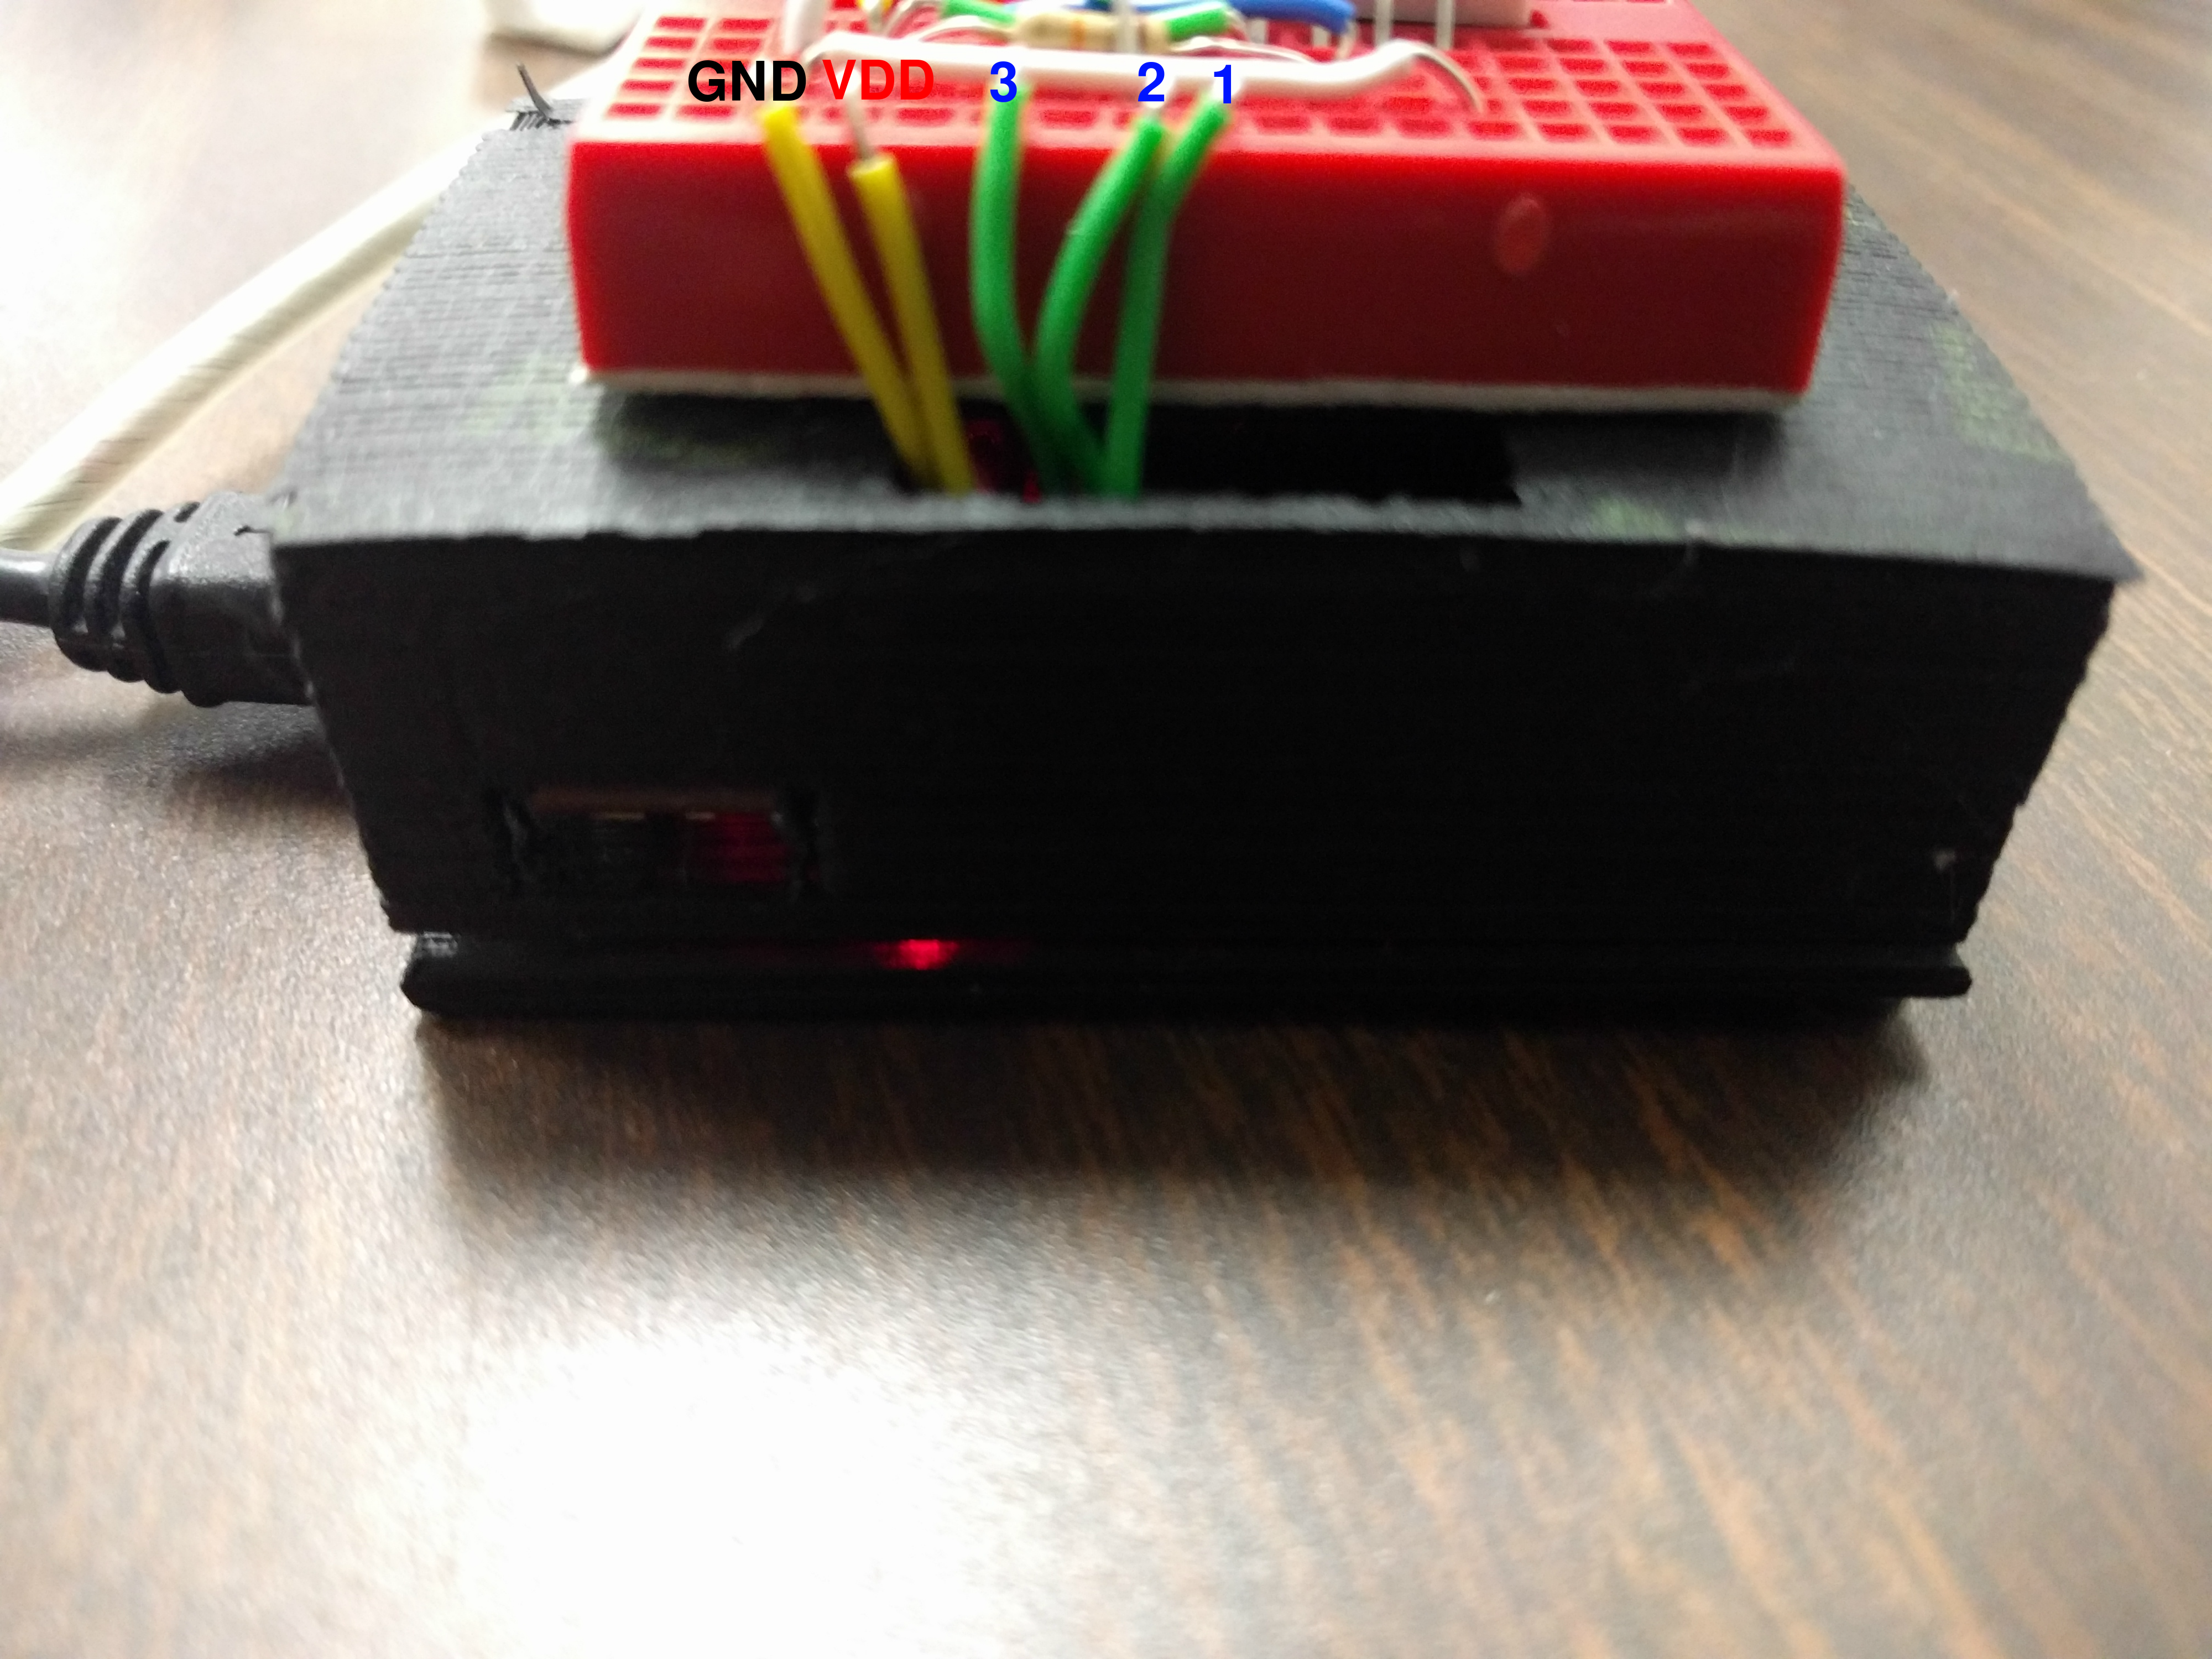
\includegraphics[scale=0.05]{images/node-pin-out.png}
  \end{center}
    \subsubsection{Job Button}
      The "Job Button" indicates when a job is complete, and starts a new job when pressed. This provides an easy way
      for a user to know when a job is completed.\\

      \textbf{Operation}\\
      Once a print is complete this button will blink repeatedly until it is pressed.  Remove the completed project,
      clean the print bed, then press the button to start the next job in the print queue.\\

      \textbf{Wiring Diagram}\\
            \begin{center}
      \includegraphics[scale=0.25]{images/job-cir.png}
      \end{center}
    \subsubsection{Temperature and Humidity}
      The temperature and humidity sensor will report the current room conditions. It
      can detect dangerous conditions for 3D printing and act as an early warning system
      if the conditions may lead to print errors.\\

      \textbf{Wiring Diagram}\\
            \begin{center}
      \includegraphics[scale=0.25]{images/temp-diagram.png}
\end{center}

    \subsubsection{Door Sensor}
      The door sensor is a magnetic switch mounted to the entrance of the printing lab.
      This allows for detection of an open or closed door, which may affect printing conditions.\\

      \textbf{Wiring Diagram}\\
      \begin{center}
        \includegraphics[scale=0.25]{images/door-cir.png}
        \end{center}
    \subsubsection{Additional Sensors}
      The nodes were set up to be universal, therefore they are compatible with
      many sensors. The nodes come with a breadboard so they can
      easily be reconfigured.\\
\newpage
  \subsection{Troubleshooting}
  \subsubsection{Reset}
  Turn the switch the the off position and unplug the node.
  \subsubsection{Node is not connecting to the hub}
  \begin{enumerate}
    \item Ensure the node has the correct wifi credentials. If the default is not
    working make sure the password hasn't been changed.
    \item If the node seems to be connected and isn't communication hard reset and re-connect.
  \end{enumerate}
  \subsubsection{Node is connected but no data is being sent from the sensors}
  Make sure the sensors are connected correctly you can reference the wiring diagrams
  in this manual.


  \newpage
    \section{Web}
  \subsection{Set up - Administrator}
  \emph{Skip this section if you are not an Adminstrator. Go to Set up - User.}\\
  \subsubsection{Adding/Deleting/Managing Users}
    Click the \textbf{User Management} menu on the left-hand side of the page.  This page will
      show you the current users, along with information about each user.\\
TODO ADD user-manage
      \begin{center}
      \includegraphics[scale=1]{images/Now-Later.png}
    \end{center}
    \begin{enumerate}
      \item \textbf{Adding a User:} Scroll down to the Add New User portion of the page.  Add the user's name,
      e-mail address, and check the box titled "Grant Admin Privileges" if you would like the user to be an
      admin.  You will receive a confirmation message below the "Users" section if successful.

      \item \textbf{Deleting a User:} Click the red trash icon under the "Actions" column to remove a user.
      You will receive a confirmation message below the "Users" section if successful.
      \begin{center}
        \includegraphics[scale=0.15]{images/control_panel_screenshots/cropped/delete_user_screenshot.png}
      \end{center}
      \item \textbf{Managing a User:} Click the yellow notepad icon under the "Actions" column to edit user
      details (Name, Email Address, or Add/Remove Admin Privileges).  Then click the "Edit User" button to confirm.
      You will receive a confirmation message below the "Users" section if successful.
      \begin{center}
        \includegraphics[scale=0.15]{images/control_panel_screenshots/full_screen/edit_user_screenshot.png}
    \end{center}
    \end{enumerate}

  \subsection{Set up - User}
      Contact your administrator and request a username and password. When they set up your account,
      you will receive an e-mail titled "Confirmation instructions".  Click the link titled \textbf{Confirm
      my account}, then login using the username and password contained in the email.  The password is case-sensitive.\\
TODO ADD login-first
      \begin{center}
      \includegraphics[scale=1]{images/Now-Later.png}
    \end{center}
      Once you have entered your username and password correctly, you will see the dashboard page.

\newpage
  \subsection{Dashboard Page}
TODO ADD dash-admin
      \begin{center}
      \includegraphics[scale=1]{images/Now-Later.png}
    \end{center}
      The Dashboard Page displays current print job information.\\
      Along the top, you will see print jobs in progress, the wait time until the job is completed, the number
      of printers that are online, and the number of printers with errors.  Click the \textbf{View Details} under
      each option to see more details, including the temperature and humidity of the room, and whether the door
      to the room is open or closed.\\
      To upload a file, either drag-and-drop the file into the box labeled \textbf{Drag N' Drop File(s)}, or
      click the \textbf{Select File} button, select the file you would like
      to print, and click the \textbf{open} button.  Your file will be uploaded to the website.


  \subsubsection{Manage Printer}
TODO ADD manage-printer
      \begin{center}
      \includegraphics[scale=1]{images/Now-Later.png}
    \end{center}
      This page shows you information about the current job, commands that were issued to the printer, a list of recent
      jobs, and the option to upload a new job.\\
      To upload a file, click the \textbf{Select File} button, select the file you would like
      to print, and click the \textbf{open} button.  Your file will be uploaded to the website.\\


  \subsubsection{Starting a Print Job}

TODO What else do we need?



  \newpage
    \section{Troubleshooting}
  \subsection{Hub or Octopi Issues}
	If you encounter difficulties with the hub or octopi, unplug them 
	from the outlet, then
       plug them back in.  The system is designed to reset itself and re-connect
       after initial set-up is completed.
  \subsection{Nodes}
  \subsubsection{How do I reset the nodes?}
     Turn the switch the the off position and unplug the node. Then plug the node back into the outlet
  and turn the switch to the on position.
  \subsubsection{Node is not connecting to the hub}
  \begin{enumerate}
    \item Ensure the node has the correct wifi credentials. If the default is not
    working make sure the password hasn't been changed.
    \item If the node seems to be connected and isn't communicating, reset the nodes.
  \end{enumerate}
  \subsubsection{Node is connected but no data is being sent from the sensors}
      Make sure the sensors are connected correctly. You can reference the wiring diagrams
     in this manual.

  \subsection{Webpage Issues}
  \subsubsection{Webpage is not loading correctly}
  \begin{enumerate}
    \item Try reloading the webpage.
    \item Try closing the webpage, then reopen the webpage.
    \item If both steps fail to fix your issue, log out of the website, then log back in.
  \end{enumerate}

  \subsection{Other Troubleshooting}
  \subsubsection{If everything else fails?}
    Turn off the node and hub by unplugging both from the outlet, then plug both back into the outlet. The system
     is designed to restart itself and reconfigure automatically once set up.
   \subsection{Acknowledgements}
	3D printer icon made by Flaticon from www.flaticon.com 


  \end{document}
